\chapter{Concepts and Architecture}
As described in the chapter Related Work, SSB is an ID-centric single feed driven environment, where onboarding is challenging. 
This prerequisite changes from the beginning. The basic idea of the Feed Bundling Protocol is to split up this ID-centric environment into replicated feed pairs, where two participants hold at least one of such a pair.  This pair contains the whole dialog between two nodes which have a contract with each other. Similar to the tin can phone from your childhood where you had two cans connected for every friend you want to communicate with. By introducing intermediary service providers, the onboarding happens at contract signing. Clients will have to possibility to connect to new servers via this ISP and create for each server a new feed pair, which is replicated over this very ISP. Since this approach means an enormous amount of feed replications between ISP and server, this feeds get bundled again.

\section{Tin Can Analogy}
This announced system seems very hard to understand but we can simplifiy it. Look at it as a tin can phone from your childhood where on either side you have two cans, strapped together for every friend you want to communicate with. You start with one corded phone to your best friend, the one you trust the most. In one you talk and the can 'saves' everything you say to it, from the other can you can only hear things from your friend, it also saves everything said from your friend. On the other side your friend has the same but can only hear things out of the one can attached to your speaking can and can only talk into the other can, which is connected to your hearing can. This are the replicated feed pairs.\\

Having this, the dialog needs a way or language to express expectations or requests from either side to communicate with each other, where you can declare what you want from each other. Leading to the simplified RPC protocol.\\

After a while it gets boring only talking to this one friend. Luckily, your friend is the coolest kid in school and knows everyone and even tells you about everyone he knows. Then you ask your friend if he could introduce you to his other friends. This introduction process closely simulates real, human social behavior.\\

After your friend has introduced you to one of his friends you and your friend start to build a new tin can phone. But because you are too far away from each other, you cannot just have a cord from one to the other, so your best friend allows you to route the cord through his house. This corresponds to the replication of the feeds over an intermediary connectivity provider.\\

But there is another problem: you are not the only one. After a while, your best friend has so many connections running through his house from all his friends who want to talk to their other friends, that here is an enormous number of strings going to that other friend. The solution is to combine all these strings into one and send all messages through this one, single bundled connection with the information into which tin can it comes at the end. He multiplexes. Given that little story, we can derive concepts and architecture for the tin can phones of the future. 
\section{Contracts}
Given that little story, we see the foundation of the friendship. The friendship between you and your best friend and the friendship between your best friend and his other friend. By the same token, it is the business contracts between the nodes that provide the foundation for the entire connectivity, protocol and bundling. These contracts are to most important building block of the whole thesis since the define the behaviour of the replicated feed pairs,  onboarding mechanics and bundling.

\subsection{Contract Values}
To build the tin can phone, three basic identifiers are needed. First of all you have to trust each other. This corresponds to the whole legal contract between the two parties. Next you need to know your names to label the phone, so you know who you are talking to. These are the public keys. \\

Since everybody in your house can use the tin phone, you also need some sort of code so that your friend knows that it is you who is sending the message and not your mother. These are the private keys. Having tha,t you need your two tin cans and two wires. One can stands for one feed and the wire for the replication. But if you do not know your friend’s address, you do not know where to put that wire, so you need that as well. 

The address, as the name is well chosen, refers to the IP-address. Last but not least, to distinguish all the cans, you label them accordingly. \\

Therefore a contract consists of actual public key, actual private key, actual feed ID and the peers public key, feed ID and location. Since a contract has been established, we need to know what happens in the tin cans and the wire. This leads to the replicated feeds.
\pagebreak

\section{Replicated Feeds}
The following sentence can be exctracted from the SSB API: ”A feed is a signed append-only sequence of messages. Each identity has exactly one feed.\footnote{\url{https://scuttlebot.io/more/protocols/secure-scuttlebutt.html}}” So what do these properties mean? 

\begin{itemize}
    \item igned message: the encryption of plain text with the sender’s private key to a cipher text. The crypto text can be deciphered with the sender’s public key. 
    \item append-only: this sequence can not be forged. So there is no possible way to modify or delete any entries that were appended at any time.\footnote{Feeds - \url{https://ssbc.github.io/scuttlebutt-protocol-guide/}} This append-only property is realized with a hash chain which references the hash value of the previously generated message.\footnote{Feeds - \url{https://ssbc.github.io/scuttlebutt-protocol-guide/}}
    \item dentity - one feed: the previously mentioned ID-centric architecture. Only one identity (key) is mapped feed, where every single bit of information you created or used in the SSB universe is stored. 
\end{itemize}
A simplified diagram can be user to illustrate that there is a lot going on in the SSB feed, but an adapted simplified version is more than sufficient for this thesis. 

\begin{figure}
    \centering
    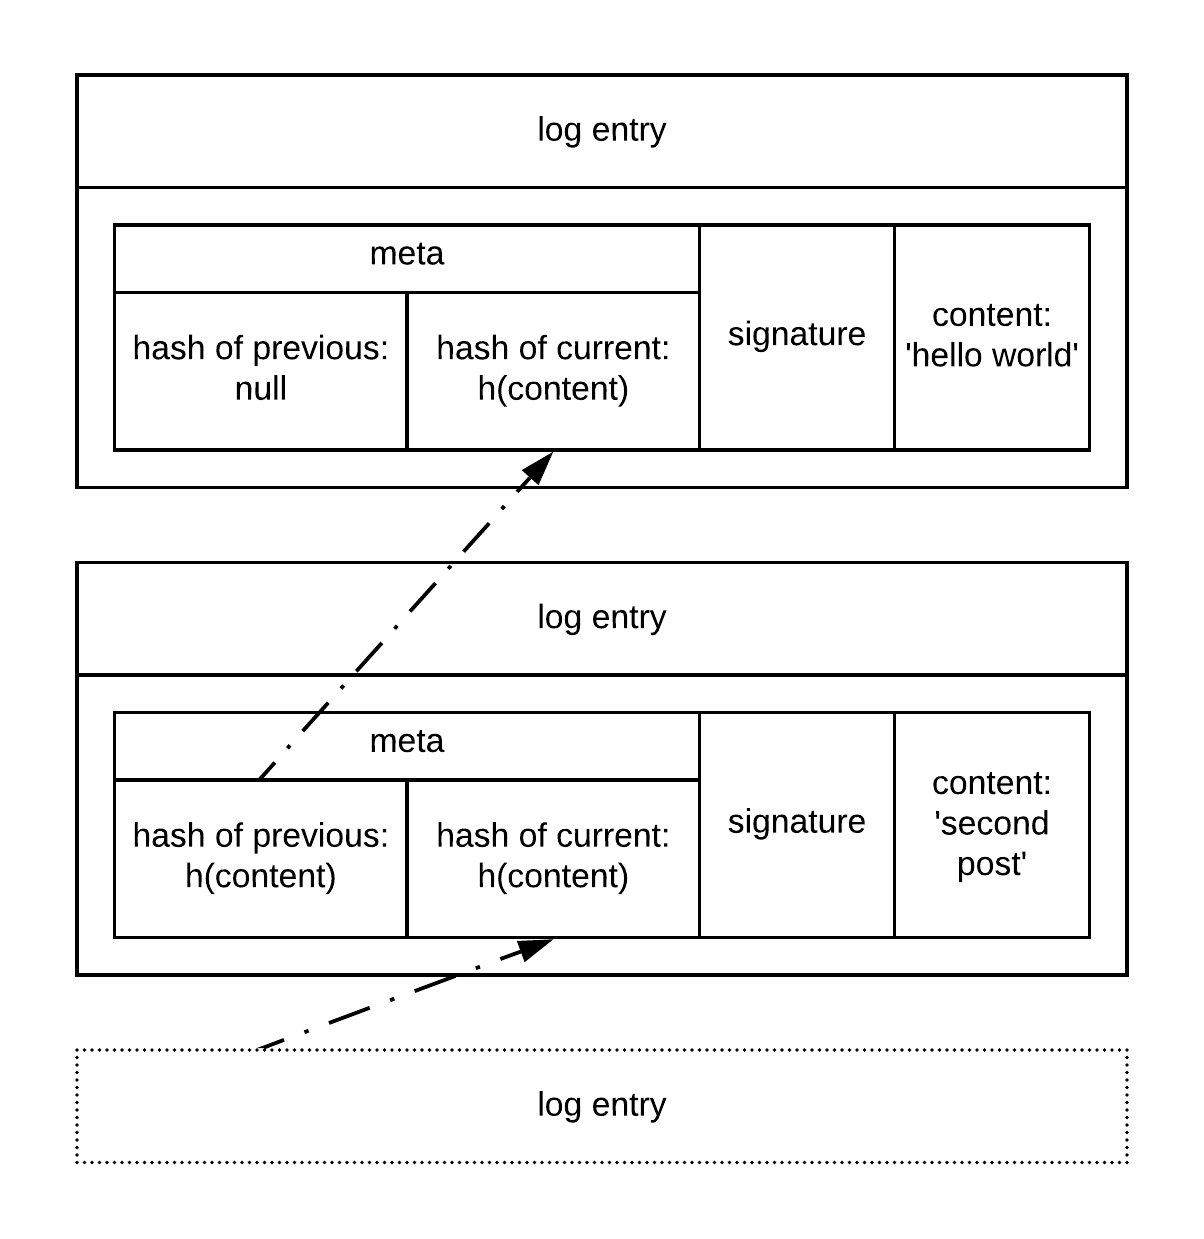
\includegraphics[width=0.5\textwidth]{feed_schema}
    \caption{A schematic simplified feed.}
    \label{fig:feed_schema}
\end{figure}
What can be derived from this information? Signing ensures that you can trust an identity. The append-only property underlines this trust by guaranteeing completeness of the information read in a feed. ID-centric feeds ensure that this feed belongs to exactly one identity, but there is the sticking point. Since the replication of the SSB protocol always replicates the whole feed to all peers (hops noch angeben) of a single identity, there is a load on the wire for big feeds. This causes latency and long scuttling time (feed update). By splitting the feeds into smaller ones, this can be bypassed and the effective communication between two parties bundled in the feed pairs mentioned previously. As a result, we have a diagram like this: For the sake of clarity, only the situation between the client and the ISP is shown. 

\begin{figure}
    \centering
    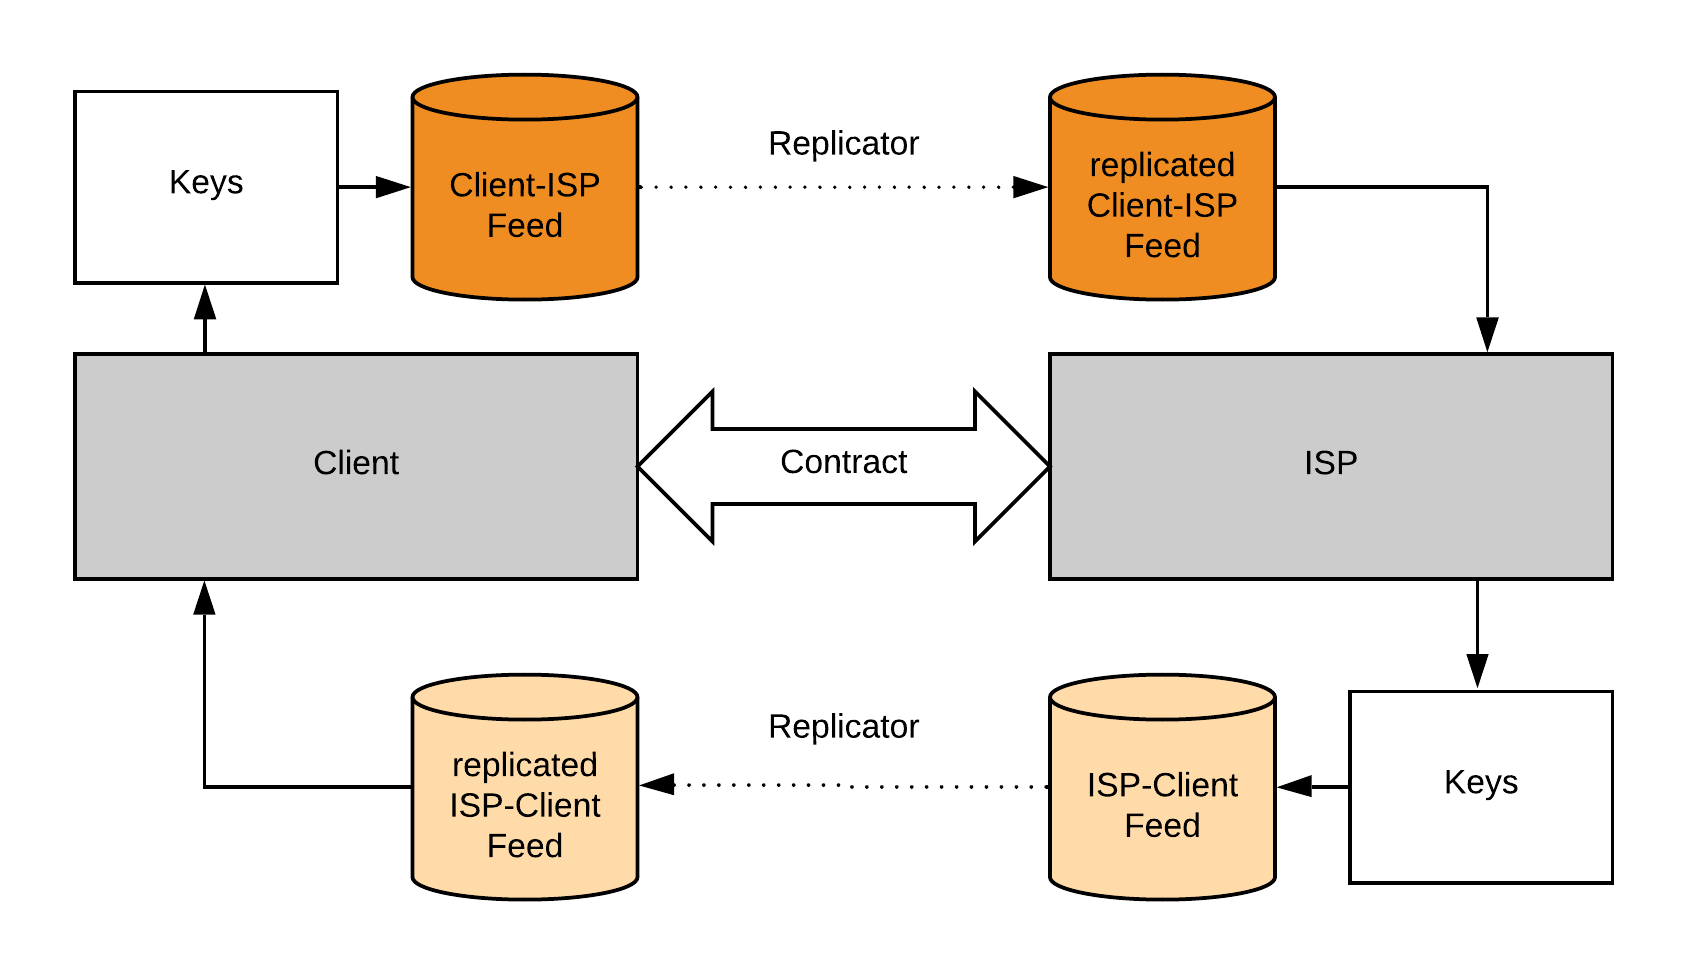
\includegraphics[width=0.9\textwidth]{fbp_v0_1_Schema}
    \caption{Full contract between client and ISP with feeds as it is the same for the server and the ISP as shown.}
    \label{fig:contract_cli_isp}
\end{figure}
The replicator or the replication process has it first appearance. As a concept, there is some sort of replicator instance or procedure that replicates the feeds to the corresponding address or location. But let’s have a closer look at the implementation part. \\
Having this setup, the next step is to have a possibility to communicate, so the client can request information from the ISP’s real database.

\pagebreak
\section{Remote Procedure Call}
As explained in the section Related Work, Remote Procedure Calls are useful paradigm for providing communication across a
network between programs.\footnote{Birrel, Nelson}. It faces many challenges, which are not important for this state of the developement of the feed bundle protocol. So the RPC used in this section is a very simplified version.\\
The Idea is to have a caller, in our case the client and a callee, the ISP or server. Having this kind of request–response protocol. An RPC is initiated by the caller, which sends a request to a callee to execute a specified procedure with given attributes. In our case these specified procedures are called services. By only having one such service e.g. the echo-service, which just echoes the attributes back to the caller we ensure the RPC-protocol works as defined. The, in the next section described, introducing and detrucing mechanics can also be summarized in such services, where the caller makes an RPC-request to the e.g. introduce-service with the needed parameters. 

%\section{v0.2}
%The next step was to include servers with services. Also here the Prerequisite and contract situation changed.
\section{Introducing and Detrucing}
\subsection{Introducing}
Recapping the tin can phone story: The idea of introducing is to get in touch with a new friend, to whom your best friend introduces you. You and your new friend create a new tin can phone. Since the cord is only long enough to reach your best friend, he connects you to your newly acquired friend. Therefore, the general idea of introducing in context of the feed bundling protocol, is onboarding to a new server over your ISP. This approach differs from the common publish and subscribe (pub-sub) architecture. Where the server has no choice to decline a client in the pub-sub model, this is the foundation of the introduce-detruce model. As we were talking of rpc before, in either way accept or decline an answer is provided to the client, else it would violate the rpc clauses.

A more detailed description: cli001 sends an RPC request to the introduce service of his ISP. This request needs an attribute which specifies the server which the client wants to be intrduced to. In this particular case ser001. isp001 invokes the introduce service, which now makes an RPC request with information about the client and the fact that it wants to introduce itself to ser001. and sends this to the server. The server has the choice to either accept or decline the introduce inquiry. If ser001 accepts the introduction, it will directly create the feed pair on its side of the two tin cans. Afterwards, it sends a confirmation or acceptance back to the ISP. Additionally to just the statement that the client was accepted the whole contract information for client is given by server: feed ID etc. 
Or the server declines the introducing approach, so the result is rejection followed by no or some sort of empty contract.

Either way isp001 gets the result and passes this result to the initial rpc request. The client now gets his result. Depending to the state of acceptance or rejection it builds its feed pair in accordance with the contract and finally the connection is successfully established. Now if client wants to use a service from server it only writes the request in the corresponding feed and the procedure is the same as described in RPC Section.
\\
An important distinction: only the client can introduce itself. The server has no knowledge of clients and also no way to acquire knowledge of clients, so only the client can ask the server for a contract. 

\subsection{Detrucing}
Detrucing as a newly invented word by me, since normally after you introduced yourself to a person there is no way to make this unhappened. It acts the same as an unfollow in a pub-sub domain. But contrary, to the introduce both parts of the contract can detruce. \\
Either client or server can send an RPC request to the ISP service to detruce, which is propagated to the opposite end descibed above in the Introducing section and results in the terminaton of the whole contract. The result of this action is deleting keys and feeds. There is no way to decline a detruce service request.
\\
An important note: after detrucing from either side, the client can yet again introduce itself to the server.
\\
A new diagram of the network can be derived using these descriptions.
\begin{figure}
    \centering
    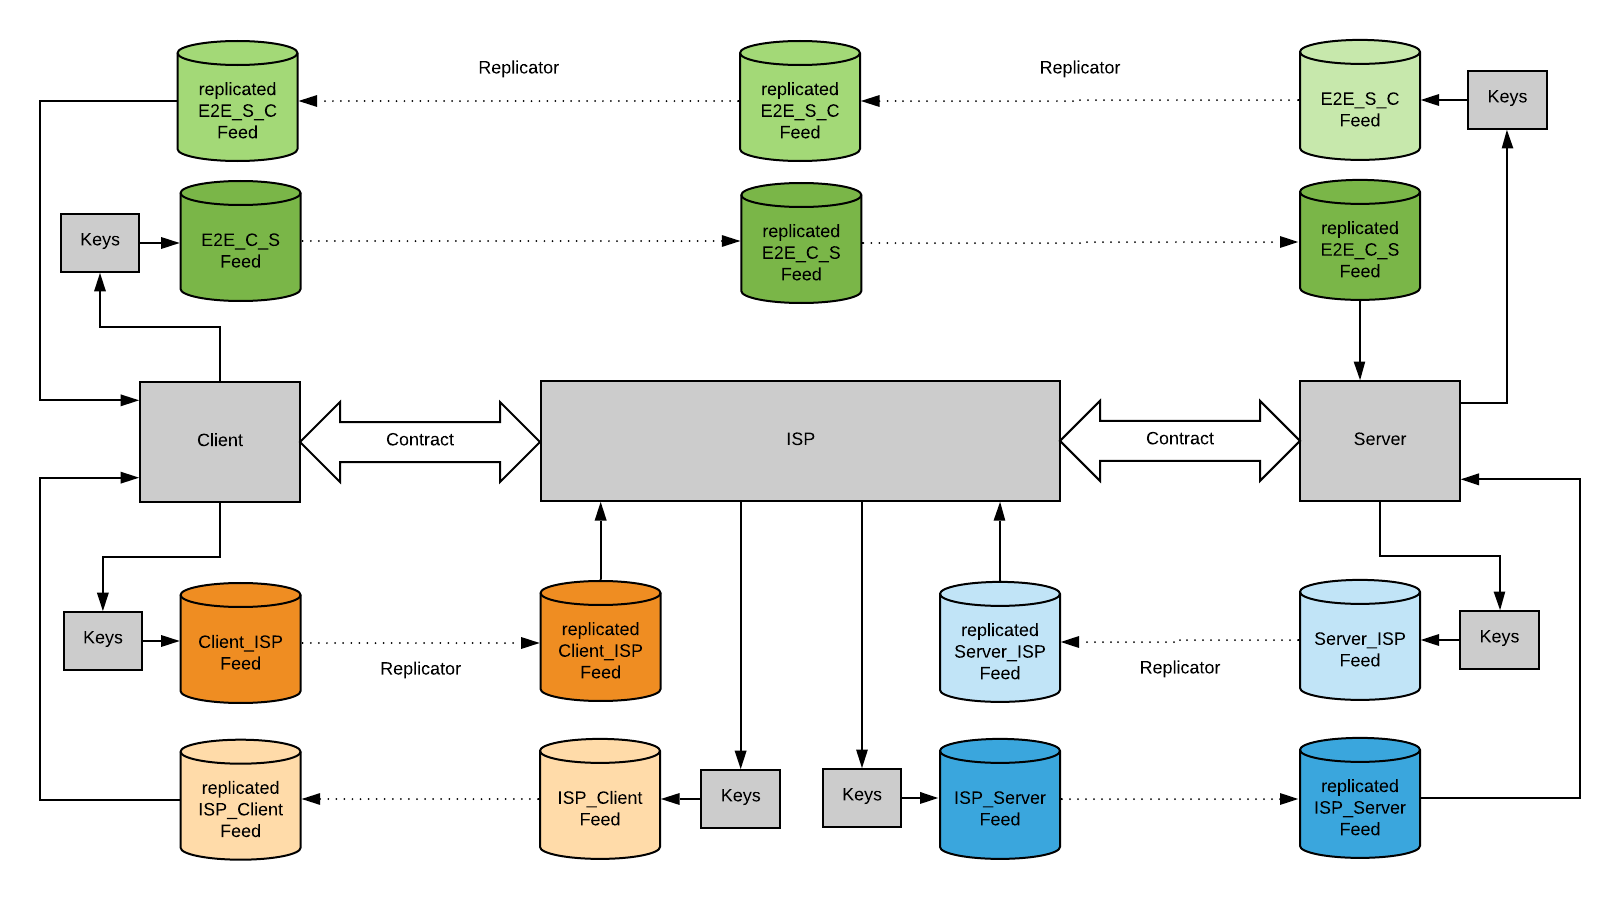
\includegraphics[width=0.9\textwidth]{intro_detru}
    \caption{State after accepted introduce from cli001 to ser001}
    \label{fig:contract_cli_isp}
\end{figure}

\pagebreak

%\section{0.4}
%added indirect communication from client to server over ISP\\
\section{Bundling}
Taking again a look at the real world problem, the ISP will have arbitrary many clients and many of them want to communicate with the same server. So instead of repeating each end to end feed pair over the ISP to the server, the new requests will be sent through a single feed pair between the ISP and server. This reduces the amount of replication work enormous.

\subsection{Adapted Introducing and Detrucing}
The introducing and detrucing idea stays the same, whereas the replication process is changed. After some server accepts a client, the server generates the whole feed pair. But instead of replicating to the ISP, nothing happens. To close the introduce request, the server sends the contract to the ISP and there the ISP generates the feed, which holds data from the server to the client. It is the same feed as in the server but it is not replicated over the general replication instance. Finally the client gets the result and generates the feed which holds the data from the client to the server. The feed pair for client-server communication gets normally replicated between client and ISP. Whereas between ISP and server a new way of replication is given.

\begin{figure}
    \centering
    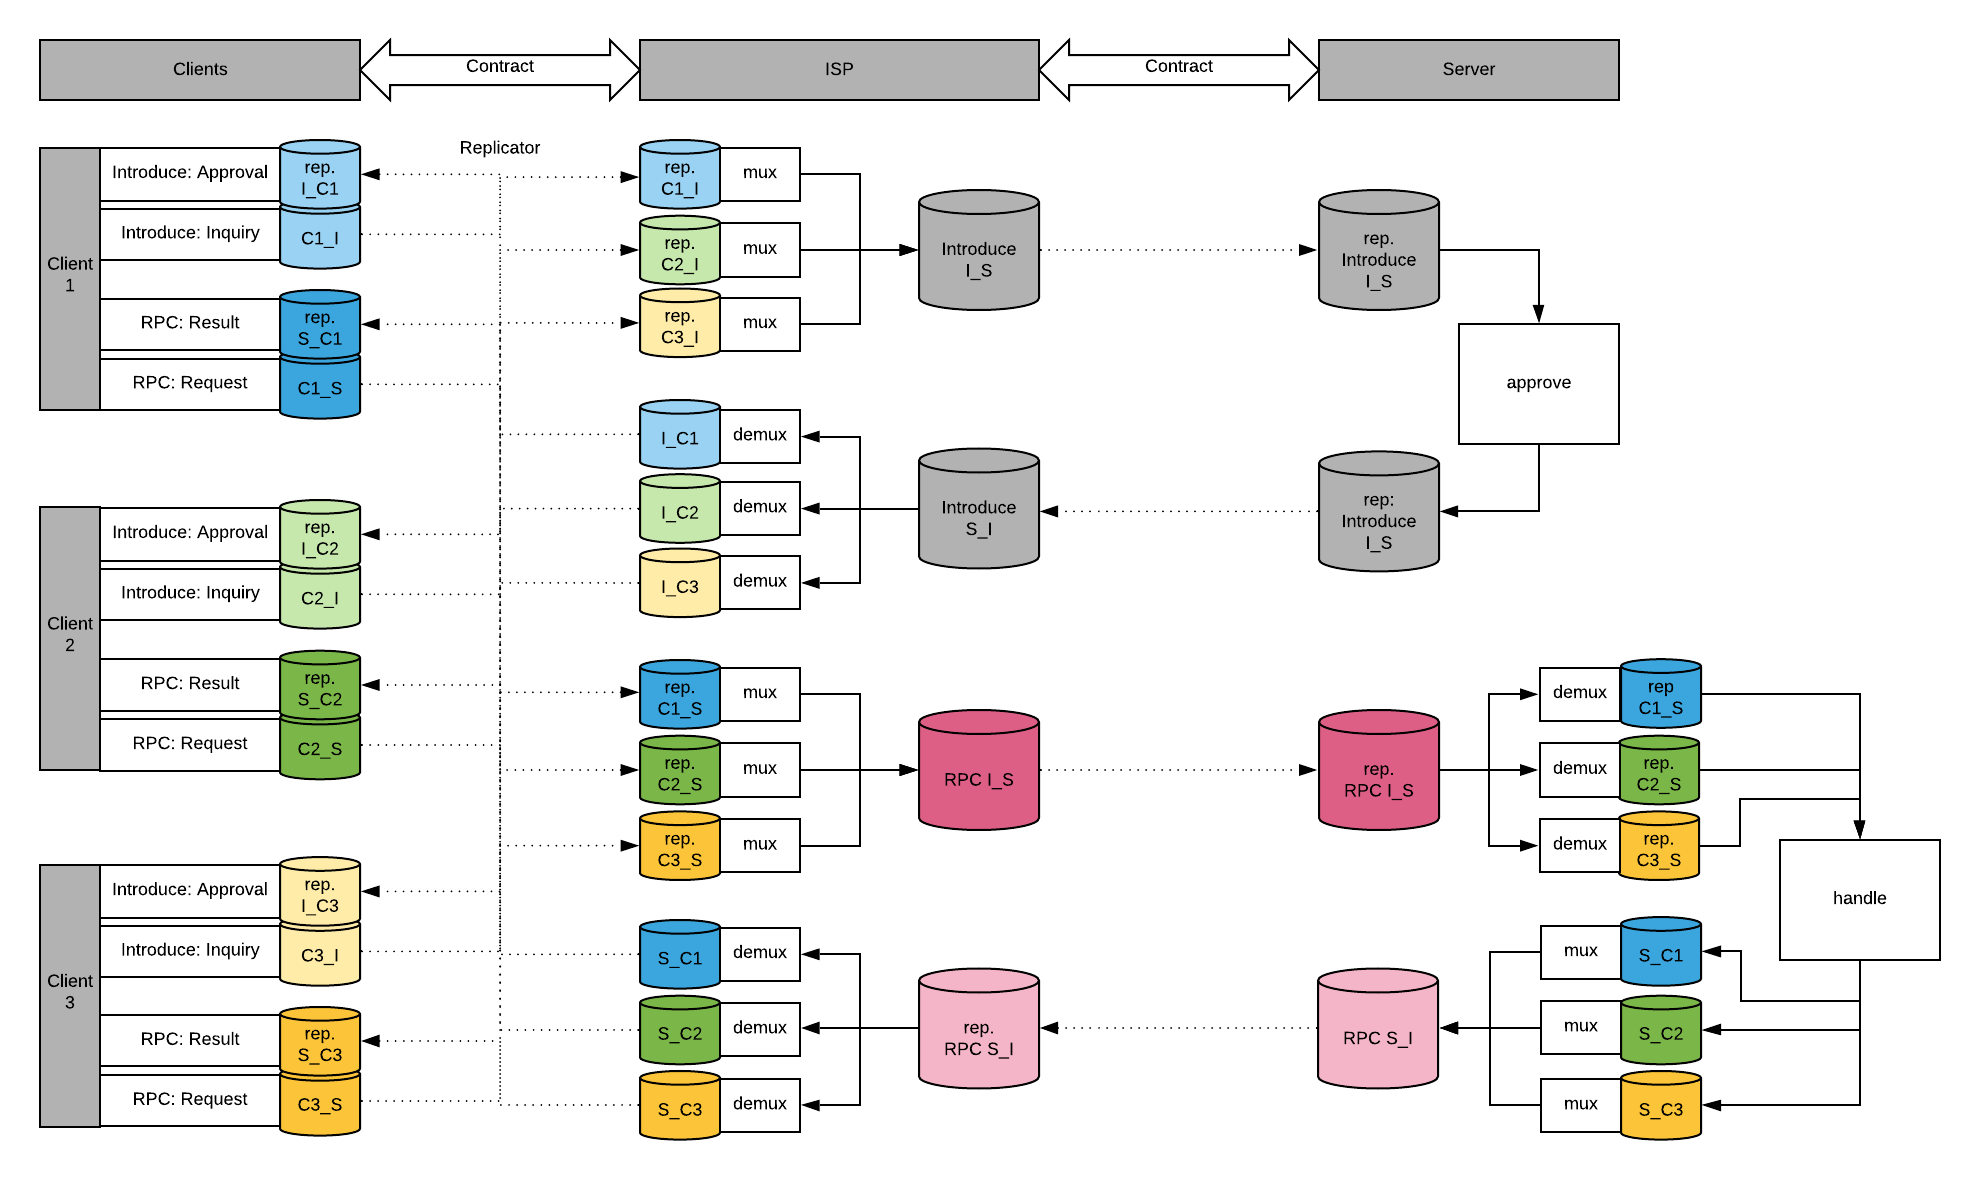
\includegraphics[width=0.9\textwidth]{mux_schema}
    \caption{multiplexing}
    \label{fig:mux}
\end{figure}

\subsection{Multiplexing and Demultiplexing}
So now we look at the communication between a client and a server. Requests from the client get transfered the same way to the ISP as before. Now instead of just forward the updated feed, by replicating to the server, the ISP detects new log entries and multiplexes these into a new log entry.
More accurate, the ISP generates a log entry signed by itself, where the content of it is the whole log entry signed by the client. This log entry is written to the ISP-server feed and replicated. The server detects the change on the ISP-server feed and takes this log entry. The multiplexed log entry, which belongs into a client-server feed is extracted and appended to the client-server feed. This step is called demultiplexing. From here we are again at the situation before. A change in the client-server feed is given and the request gets handled. The result is written to the server-client feed and again not replicated. From there the whole story is repeated. The log entry gets again multiplexed in the server-ISP feed. At the ISP the log entry is demultiplexed and appended to the server-client feed. From there it is replicated to the client and the client got its result for the request.

\textit{Schema von log entry in log entry}


\section{Outlook}
Having all these concepts and architecture, we see the whole process is simplified on a single central ISP. In the real world this is not the case, hence as prove of concept it is more than enough. In the next steps the system has to be expanded by splitting this very ISP into a net of ICPs. They act as as effective connectivity stations and an architecture has to be found where clients and servers connect to these conectivity nodes. Also adding more ISPs, more companies is needed. The dynamic of contracts between ISPs has to be explored, but more in the Future Work section.